\titleformat{\section}{\centering\normalfont\fontsize{20}{25}\bfseries}{\thesection}{1em}{}
\appendix
%\pagenumbering{Roman}
%\setcounter{page}{1}
%\topskip0pt
\vspace*{\fill}
\renewcommand{\thesection}{} %% Here we redefine the chapter counter
\section{Appendix}
\label{chap:appendix}
\renewcommand{\thesection}{\Alph{section}} %%And here we redefine it back
\renewcommand{\thesubsection}{\Alph{subsection}}
\vspace{\fill}

\counterwithin{figure}{section}
\counterwithin{table}{section}
\setcounter{table}{0}
\setcounter{figure}{0}

\fakesubsection{Tables}
\label{apdx:tables}

\begin{table*}[p]
    \begin{center}
    \caption{Rhyme Densities}
    \vspace{6pt}
    \label{tab:complete-rd-table}
    \bgroup
    \def\arraystretch{1.3}
    \resizebox{7.9cm}{!}{
    \begin{tabular}{c|l|c}
        Rank & \multicolumn{1}{c|}{Artist} & Rhyme Density \\[0.1cm]\hline
        1. & Earl Sweatshirt & 1.217 \\
        2. & Montana of 300 & 1.210 \\
        3. & Joey Badass & 1.167 \\
        4. & ASAP Rocky & 1.158 \\
        5. & Action Bronson & 1.151 \\
        6. & Bas & 1.138 \\
        7. & Mac Miller & 1.129 \\
        8. & Isaiah Rashad & 1.123 \\
        9. & Deniro Farrar & 1.123 \\
        10. & Logic & 1.123 \\
        11. & ASAP Ant & 1.122 \\
        12. & Big L & 1.117 \\
        13. & CunninLynguists & 1.109 \\
        14. & Lil Wayne & 1.108 \\
        15. & Royce Da 59 & 1.098 \\
        16. & Nas & 1.097 \\
        17. & Eminem & 1.093 \\
        18. & Common & 1.090 \\
        19. & The Notorious B.I.G  & 1.066 \\
        20. & Tupac & 1.066 \\
        21. & Talib Kweli & 1.059 \\
        22. & Kayne West & 1.056 \\
        23. & Chance The Rapper & 1.051 \\
        24. & Jay-Z & 1.050 \\
        25. & J Cole & 1.049 \\
        26. & Scarface & 1.049 \\
        27. & Pusha T & 1.049 \\
        28. & NF & 1.034 \\
        29. & Lupe Fiasco & 1.032 \\
        30. & Eazy-E & 1.021 \\
        31. & Drake & 1.020 \\
        32. & Kendrick Lamar & 1.019 \\
        33. & Childish Gambino & 1.001 \\
        34. & Tyler The Creator & 0.998 \\
        35. & Immortal Technique & 0.998 \\
        36. & Ice Cube & 0.924 \\
        37. & Andre 3000 & 0.883 \\\hline
        \multicolumn{2}{c|}{Mean Rhyme Density:} & 1.074.27 \\
        \hline
    \end{tabular}
    }
    \egroup
    \end{center}
\end{table*}

\begin{table*}[p]
    \begin{center}
    \caption{Examples of Lyric Generation Using Different Sampling Techniques with Optimized Parameters}
    \vspace{5pt}
    \resizebox{15cm}{!}{
    \bgroup
    \renewcommand\cellset{\renewcommand\arraystretch{1.13}}
    \def\arraystretch{1.8}
    \label{tab:lyric-generation-examples}
    \begin{tabular}{m{4cm}|m{10cm}}
        \multicolumn{1}{c}{\textbf{Configuration}} & \multicolumn{1}{c}{\textbf{Generated Lyrics}}
        \\\hline\hline
        \makecell[c]{Greedy Search} &
        {\em \makecell[l]{
        i want to get the police but i can't stop the same \\
        i don't know what i wanna do \\
        i don't know what i wanna do \\
        i don't know what i wanna do \\
        i don't know what i wanna do \\
        i don't know what i wanna d}} \\\hline
        
        \makecell[c]{Temperature Sampling \\ $t=0.7$} &
        {\em \makecell[l]{
        i freedom with the lights in the parking lane \\
        i got all the beat i make it work, they can't do my time \\
        it's all about you \\
        you know you're so cold, you don't really need \\
        to deal with you, you cree}} \\\hline
        
        \makecell[c]{Beam Search \\ $\beta=2$} &
        {\em \makecell[l]{
        i want to tell you about it, i was the one that i know \\
        and i know it's just the way i escape \\
        yeah, i said it all falls down \\
        i don't know what to do \\
        they wonder why i never get tight \\
        i don't want}} \\\hline
        
        \makecell[c]{Top-k Sampling \\ $k=2, t=0.6$} &
        {\em \makecell[l]{
        the cards,it though, tou still are \\
         it's a struggle to be a presing road \\
         to things,inder to get these propers \\
         i came torolicing, thank the familiar \\
         sthat i'm a sang to shart, \\
         in an end and, i'm a m}} \\\hline
         
         \makecell[c]{Top-k Sampling \\ $k=2, t=0.7$} &
        {\em \makecell[l]{
        i would trave a life, i can't stay to say than i'm sorry \\
        ii'm a real nice an enemy,in any merming on the streets \\
        i'm trynna beath in the country anywar i got anothar \\
        and i aim't nervous, i'masteleg}} \\\hline
        
        \makecell[c]{Top-p Sampling \\ $p=0.64$} &
        {\em \makecell[l]{
        this a dick that was made in shows of his crew \\
        and so what the fuck is time? \\
        and he gon' make you a pick of niggas in a house rap \\
        some girl get a place to battle the walls like this \\
        been a baby a}} \\\hline
        
        \makecell[c]{Top-p Sampling \\ $p=0.68$} &
        {\em \makecell[l]{
        i'm lookin' for some new leaders ow my granny mary \\
        my drug palling my heart serming up \\
        no too long to be all the shit i do \\
        i think i'll take it back to common tell \\
        they say the world that say the}} \\\hline
        
        \makecell[c]{Top-p Sampling \\ $p=0.74$} &
        {\em \makecell[l]{
        lord willin', baby i'm happy when i see the lowl \\
        you gettin' contented, i'm feelin' tripping on a disc \\
        yeah, this is sore than i con't have it \\
        my mind be driving my back, love to say my fucking wi}}
        \\\hline \multicolumn{2}{l}{* Lyrics generated at seed = 42/500}
    \end{tabular}
    \egroup
    }
    \end{center}
\end{table*}

\begin{table*}[p]
    \begin{center}
    \caption{Beam Search Parameter Exploration}
    \vspace{6pt}
    \bgroup
    \def\arraystretch{1.3}
    \label{tab:beam-param-eval}
    \begin{tabular}{|c|c|c|}
        \hline
        \textbf{Stage} & \textbf{Beam width ($\beta$)} & \textbf{Iterations} \\\hline \hline
        1. & $[2 \ldots 10], s=1$ & $20V \cdot 200C$ \\\hline
        2. & $\{2, 3, 4\}, s=1$ & $60V \cdot 200C$ \\\hline
        FINAL & \textbf{2} & \textit{N/A}
        \\\whline
    \end{tabular}
    \egroup
    \end{center}
\end{table*}

\begin{table*}[p]
    \begin{center}
    \caption{Temperature Sampling Parameter Exploration}
    \vspace{6pt}
    \bgroup
    \def\arraystretch{1.3}
    \label{tab:tempparameval}
    \begin{tabular}{|c|c|c|}
        \hline
        \textbf{Stage} & \textbf{Temperature (T)} & \textbf{Iterations} \\\hline\hline
        1. & $[0.1 \ldots 1.2], s=0.1$ & $20V \cdot 200C$ \\\hline
        2. & $[0.5 \ldots 0.9], s=1$ & $60V \cdot 200C$ \\\hline
        FINAL & \textbf{0.7} & \textit{N/A}
        \\\whline
    \end{tabular}
    \egroup
    \end{center}
\end{table*}

\begin{table*}[p]
    \begin{center}
    \caption{Top-k Sampling Parameter Exploration}
    \vspace{6pt}
    \bgroup
    \def\arraystretch{1.3}
    \label{tab:top-k-param-eval}
    \begin{tabular}{|c|c|c|c|}
        \hline
        \textbf{Stage} & \textbf{Temperature (T)} & \textbf{Top-k value} & \textbf{Iterations} \\\hline\hline
        1. & $[0.1 \ldots 1.2], s=0.1$ & $[2 \ldots 6], s=1$ & $20V \cdot 200C$ \\\hline
        2. & $[0.1 \ldots 1.2], s=0.1$ & \{2, 3\} & $60V \cdot 200C$ \\\hline
        FINAL & \{\textbf{0.6, 0.7}\} & \textbf{2} & \textit{N/A}
        \\\whline
    \end{tabular}
    \egroup
    \end{center}
\end{table*}

\begin{table*}[p]
    \begin{center}
    \caption{Top-p Sampling Parameter Exploration}
    \vspace{6pt}
    \bgroup
    \def\arraystretch{1.3}
    \label{tab:top-p-param-eval}
    \begin{tabular}{|c|c|c|}
        \hline
        \textbf{Stage} & \textbf{Top-p value} & \textbf{Iterations} \\\hline\hline
        1. & $[0.90 \ldots 0.99], s=0.01$ & $60V \cdot 200C$ \\\hline
        2. & $[0.80 \ldots 0.89], s=0.01$ & $60V \cdot 200C$ \\\hline
        3. & $[0.70 \ldots 0.79], s=0.01$ & $60V \cdot 200C$ \\\hline
        4. & $[0.50 \ldots 0.68], s=0.02$ & $60V \cdot 200C$ \\\hline
        FINAL & \{\textbf{0.64, 0.68, 0.74}\} & \textit{N/A}
        \\\whline
    \end{tabular}
    \egroup
    \end{center}
\end{table*}

\begin{table*}[p]
    \begin{center}
    \caption{Eminem: "Lose Yourself" Lyrics}
    \vspace{6pt}
    \bgroup
    \renewcommand\cellset{\renewcommand\arraystretch{1.13}}
    \def\arraystretch{1.5}
    \label{tab:lose-yourself-lyrics}
    \begin{tabular}{|c|c p{11.3cm}|}
        \hline
        \textbf{Type} & \multicolumn{2}{|c|}{\textbf{Lyrics}} \\\hline \hline
        \makecell[c]{Intro} & \makecell[c]{1 \\ 2 \\ 3 \\ 4} &
        {\em \makecell[l]{
        Look, if you had, one shot, or one opportunity \\
        To seize everything you ever wanted, in one moment \\
        Would you capture it, or just let it slip? \\
        Yo}} \\\hline
        \makecell[c]{Verse(1)} & \makecell[c]{5 \\ 6 \\ 7 \\ 8 \\ 9 \\ 10 \\ 11 \\ 12 \\ 13 \\ 14 \\ 15 \\ 16 \\ 17 \\ 18 \\ 19 \\ 20} &
        {\em \makecell[l]{
        His palms are sweaty, knees weak, arms are heavy \\
        There's vomit on his sweater already, mom's spaghetti \\
        He's nervous, but on the surface he looks calm and ready \\
        To drop bombs, but he keeps on forgetting \\
        What he wrote down, the whole crowd goes so loud \\
        He opens his mouth, but the words won't come out \\
        He's choking, how? Everybody's joking now \\
        The clock's run out, time's up, over, blaow \\
        Snap back to reality, ope there goes gravity, ope \\
        There goes Rabbit, he choked, he's so mad but he won't \\
        Give up that easy, no, he won't have it, he knows \\
        His whole back's to these ropes, it don't matter, he's dope \\
        He knows that but he's broke, he's so stagnant, he knows \\
        When he goes back to this mobile home, that's when it's \\
        Back to the lab again, yo, this old rhapsody \\
        Better go capture this moment and hope it don't pass him, and \\
        }} \\\hline
        \makecell[c]{Chorus(x2)} & \makecell[c]{21 \\ 22 \\ 23 \\ 24 \\ 25} &
        {\em \makecell[l]{
        You better lose yourself in the music \\
        The moment, you own it, you better never let it go (Go) \\
        You only get one shot, do not miss your chance to blow \\
        This opportunity comes once in a lifetime, yo \\
        You better… \\
        }} \\\hline
        \makecell[c]{Verse(2)} & \makecell[c]{26 \\ 27 \\ 28 \\ 29 \\ 30 \\ 31 \\ 32 \\ 33 \\ 34 \\ 35 \\ 36 \\ 37 \\ 38 \\ 39 \\ 40 \\ 41} &
        {\em \makecell[l]{
        His soul's escaping through this hole that is gaping \\
        This world is mine for the taking, make me king \\
        As we move toward a New World Order \\
        A normal life is boring; but superstardom's \\
        Close to post-mortem, it only grows harder \\
        Homie grows hotter, he blows, it's all over \\
        These hoes is all on him, coast-to-coast shows \\
        He's known as the Globetrotter, lonely roads \\
        God only knows, he's grown farther from home, he's no father \\
        He goes home and barely knows his own daughter \\
        But hold your nose, 'cause here goes the cold water \\
        These hoes don't want him no more, he's cold product \\
        They moved on to the next schmoe who flows \\
        He nose-dove and sold nada, and so the soap opera \\
        Is told, it unfolds, I suppose it's old, partner \\
        But the beat goes on, da-da-dom, da-dom, dah-dah, dah-dah \\
        }} \\\hline
    \end{tabular}
    \egroup
    \end{center}
\end{table*}

\begin{table*}[p]
    \begin{center}
    \vspace{6pt}
    \bgroup
    \renewcommand\cellset{\renewcommand\arraystretch{1.13}}
    \def\arraystretch{1.5}
    \begin{tabular}{|c|c p{11.3cm}|}
        \hline
        \makecell[c]{Chorus(x2)} & \makecell[c]{42 \\ 43 \\ 44 \\ 45 \\ 46} &
        {\em \makecell[l]{
        You better lose yourself in the music \\
        The moment, you own it, you better never let it go (Go) \\
        You only get one shot, do not miss your chance to blow \\
        This opportunity comes once in a lifetime, yo \\
        You better… \\
        }} \\\hline
        \makecell[c]{Verse(3)} & \makecell[c]{47 \\ 48 \\ 49 \\ 50 \\ 51 \\ 52 \\ 53 \\ 54 \\ 55 \\ 56 \\ 57 \\ 58 \\ 59 \\ 60 \\ 61 \\ 62 \\ 63 \\ 64 \\ 65 \\ 66 \\ 67 \\ 68 \\ 69} &
        {\em \makecell[l]{
        No more games, I'ma change what you call rage \\
        Tear this motherfuckin' roof off like two dogs caged \\
        I was playin' in the beginning, the mood all changed \\
        I've been chewed up and spit out and booed off stage \\
        But I kept rhymin' and stepped right in the next cypher \\
        Best believe somebody's payin' the Pied Piper \\
        All the pain inside amplified by the \\
        Fact that I can't get by with my nine-to- \\
        Five and I can't provide the right type of life for my family \\
        'Cause man, these goddamn food stamps don't buy diapers \\
        And there's no movie, there's no Mekhi Phifer, this is my life \\
        And these times are so hard, and it's gettin' even harder \\
        Tryna feed and water my seed, plus teeter-totter \\
        Caught up between bein' a father and a prima donna \\
        Baby mama drama, screamin' on her, too much for me to wanna \\
        Stay in one spot, another day of monotony's \\
        Gotten me to the point I'm like a snail, I've got \\
        To formulate a plot or end up in jail or shot \\
        Success is my only motherfuckin' option, failure's not \\
        Mom, I love you, but this trailer's got \\
        To go; I cannot grow old in Salem's Lot \\
        So here I go, it's my shot, feet, fail me not \\
        This may be the only opportunity that I got \\
        }}\\\hline
        \makecell[c]{Chorus(x2)} & \makecell[c]{70 \\ 71 \\ 72 \\ 73 \\ 74} &
        {\em \makecell[l]{
        You better lose yourself in the music \\
        The moment, you own it, you better never let it go (Go) \\
        You only get one shot, do not miss your chance to blow \\
        This opportunity comes once in a lifetime, yo \\
        You better… \\
        }} \\\hline
        \makecell[c]{Outro} & \makecell[c]{75} &
        {\em \makecell[l]{
        You can do anything you set your mind to, man \\
        }} \\\hline
    \end{tabular}
    \egroup
    \end{center}
\end{table*}

\pagebreak

\fakesubsection{Figures}
\label{apdx:figures}

\begin{figure*}[h]
    \centering
    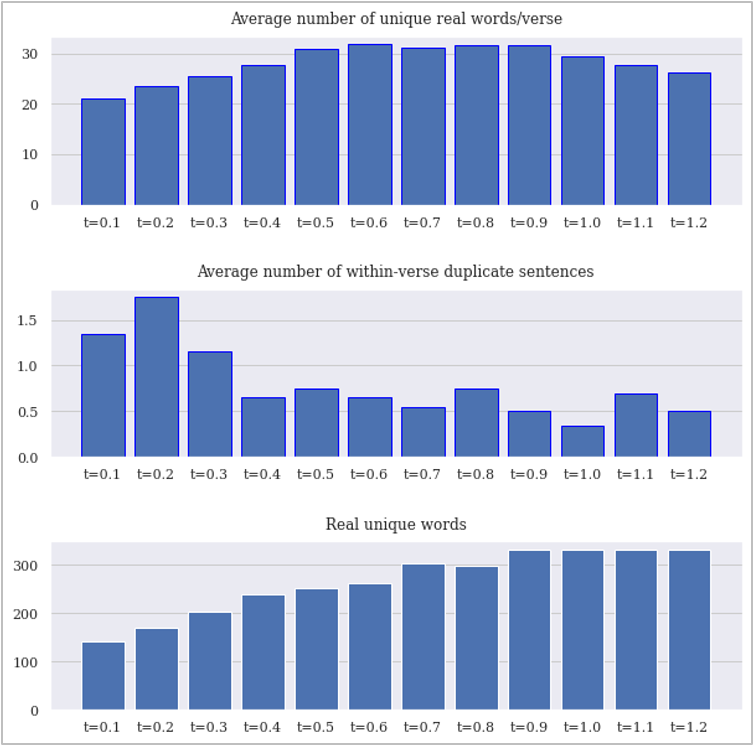
\includegraphics[scale=0.70, keepaspectratio=true]{figures/temp_param_eval_s1.png}
    \caption{Temperature Sampling Parameter Evaluation Metrics (Stage 1/2)}
    \label{fig:temp-param-eval-1}
\end{figure*}

\begin{figure*}[h]
    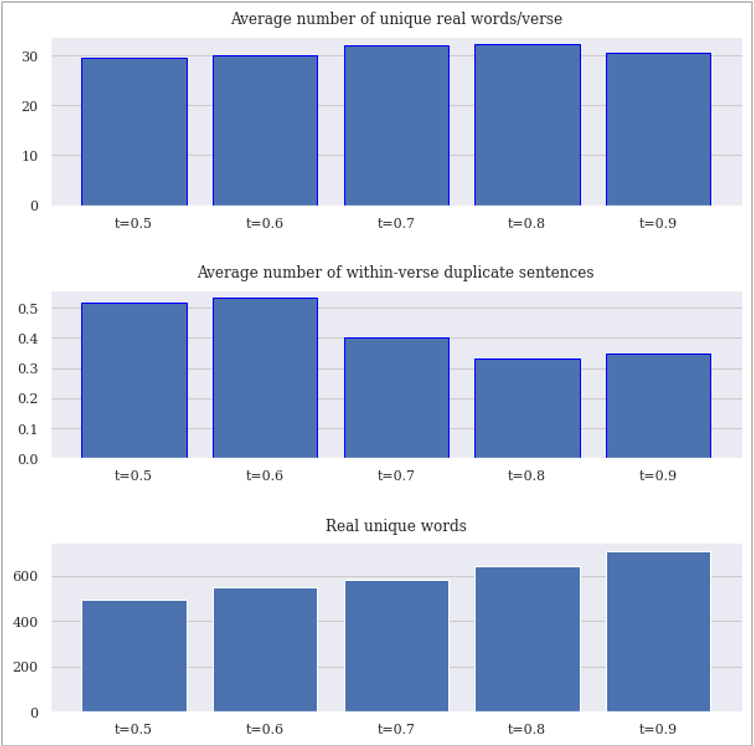
\includegraphics[width=\textwidth, height=\textheight,keepaspectratio=true]{figures/temp_param_eval_s2.png}
    \caption{Temperature Sampling Parameter Evaluation Metrics (Stage 2/2)}
    \label{fig:temp-param-eval-2}
\end{figure*}

\begin{figure*}[h]
    \centering
    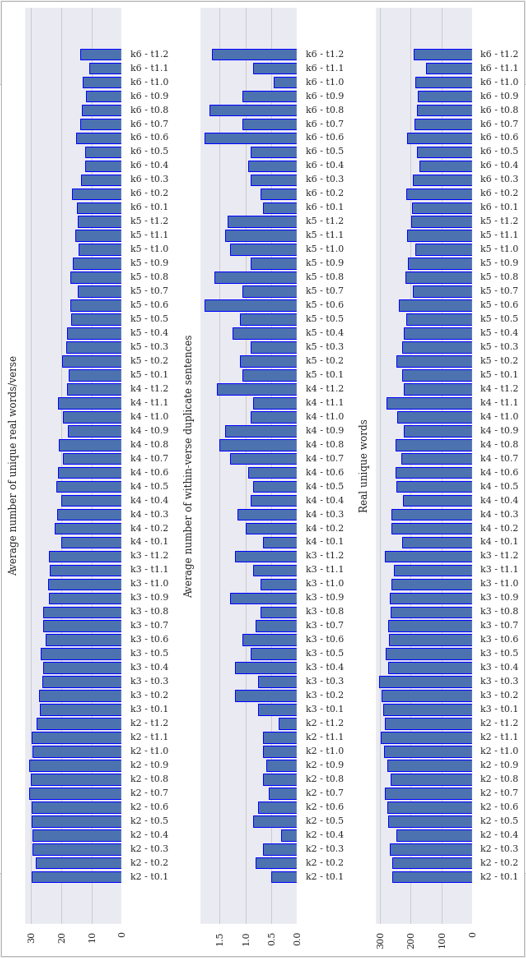
\includegraphics[scale=0.85, keepaspectratio=true]{figures/top-k_param_eval_s1.png}
    \caption{Top-k Sampling Parameter Evaluation Metrics (Stage 1/2)}
    \label{fig:top-k-param-eval-1}
\end{figure*}

\begin{figure*}[h]
    \centering
    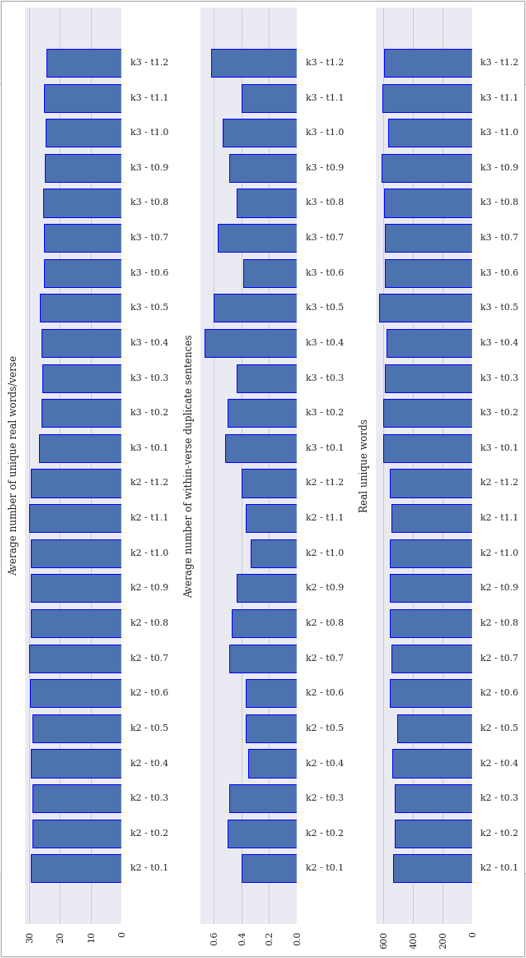
\includegraphics[scale=0.85,keepaspectratio=true]{figures/top-k_param_eval_s2_1.png}
    \caption{Top-k Sampling Parameter Evaluation Metrics (Stage 2/2) v1}
    \label{fig:top-k-param-eval-s2-v1}
\end{figure*}

\begin{figure*}[h]
    \centering
    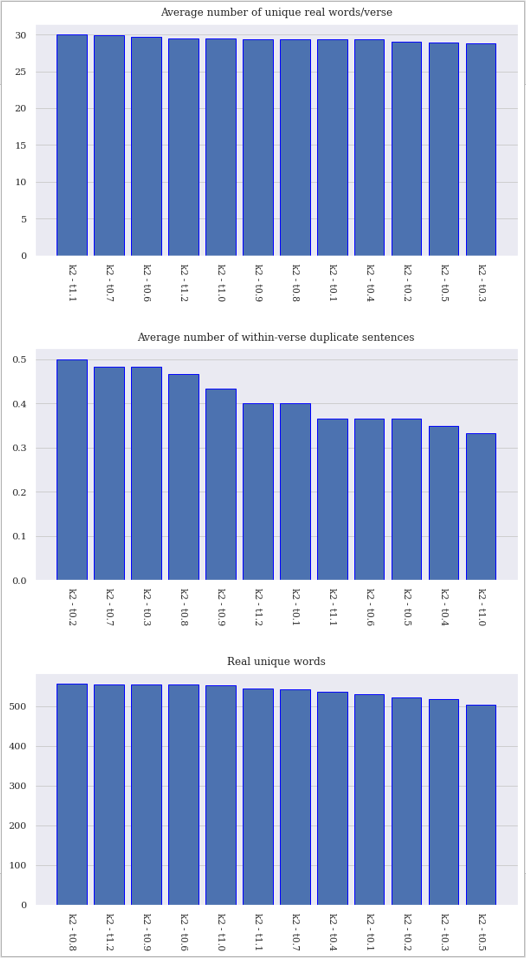
\includegraphics[scale=0.85,keepaspectratio=true]{figures/top-k_param_eval_s2_2.png}
    \caption{Top-k Sampling Parameter Evaluation Metrics (Stage 2/2) v2 - Sorted according to values in descending order}
    \label{fig:top-k-param-eval-s2-v2}
\end{figure*}

\begin{figure*}[h]
    \centering
    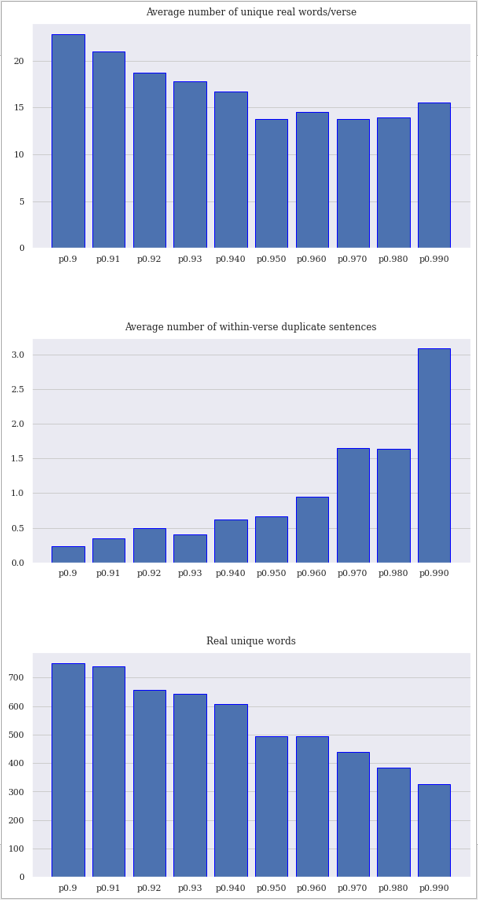
\includegraphics[scale=0.85,keepaspectratio=true]{figures/top-p_param_eval_s1.png}
    \caption{Top-p Sampling Parameter Evaluation Metrics (Stage 1/4)}
    \label{fig:top-p-param-eval-s1}
\end{figure*}

\begin{figure*}[h]
    \centering
    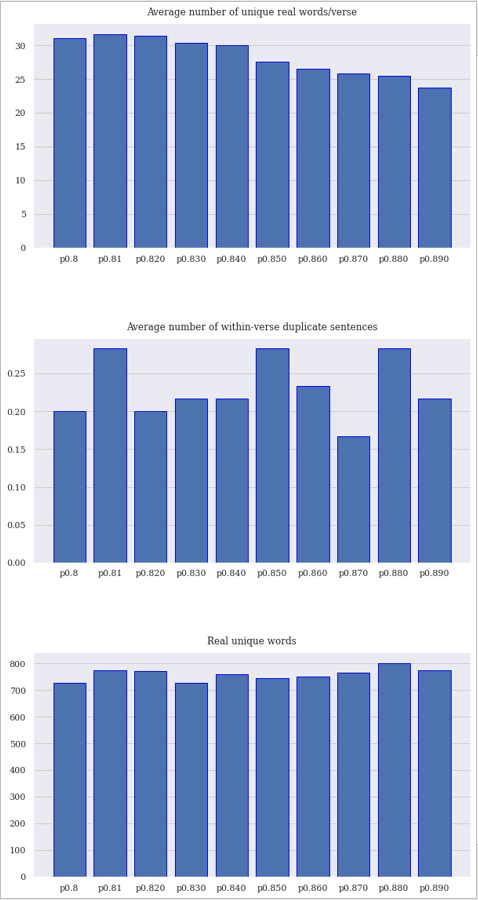
\includegraphics[scale=0.85,keepaspectratio=true]{figures/top-p_param_eval_s2.png}
    \caption{Top-p Sampling Parameter Evaluation Metrics (Stage 2/4)}
    \label{fig:top-p-param-eval-s2}
\end{figure*}

\begin{figure*}[h]
    \centering
    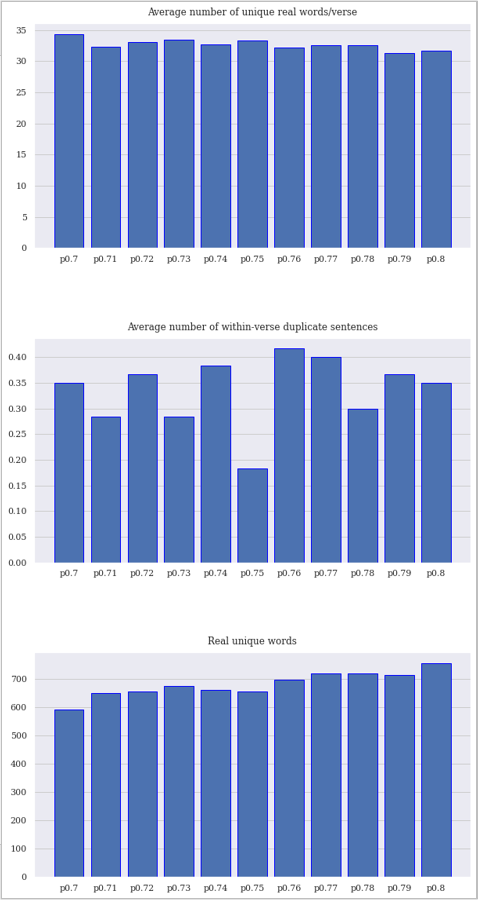
\includegraphics[scale=0.85,keepaspectratio=true]{figures/top-p_param_eval_s3.png}
    \caption{Top-p Sampling Parameter Evaluation Metrics (Stage 3/4)}
    \label{fig:top-p-param-eval-s3}
\end{figure*}

\begin{figure*}[h]
    \centering
    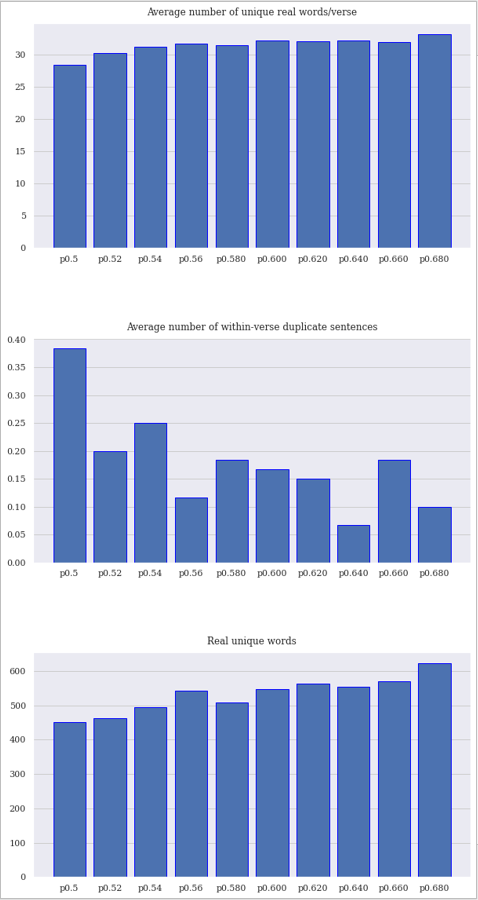
\includegraphics[scale=0.85,keepaspectratio=true]{figures/top-p_param_eval_s4.png}
    \caption{Top-p Sampling Parameter Evaluation Metrics (Stage 4/4)}
    \label{fig:top-p-param-eval-s4}
\end{figure*}

\begin{figure*}[h]
    \centering
    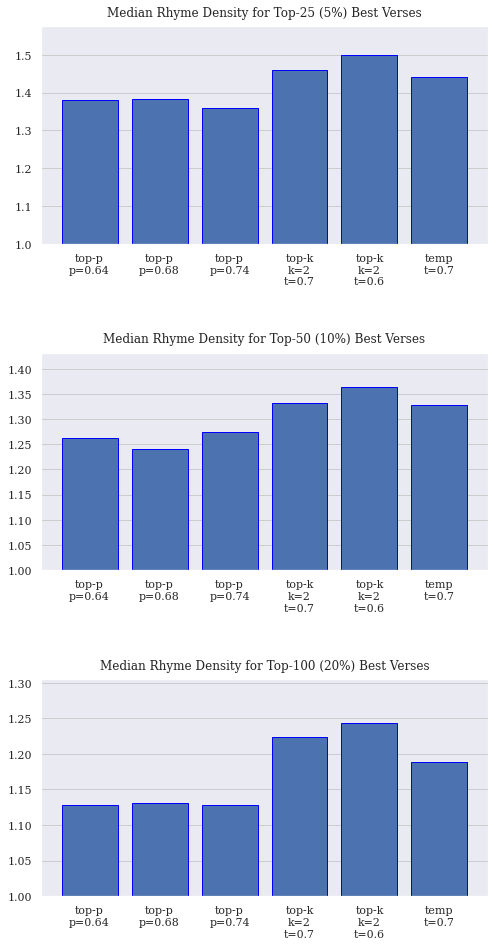
\includegraphics[scale=0.64, keepaspectratio=true]{figures/top_verse_rd_median.png}
    \caption{Median Rhyme Density for Top-25, Top-50 and Top-100 Best Verses}
    \label{fig:top_rd_median}
\end{figure*}

\begin{figure*}[h]
    \centering
    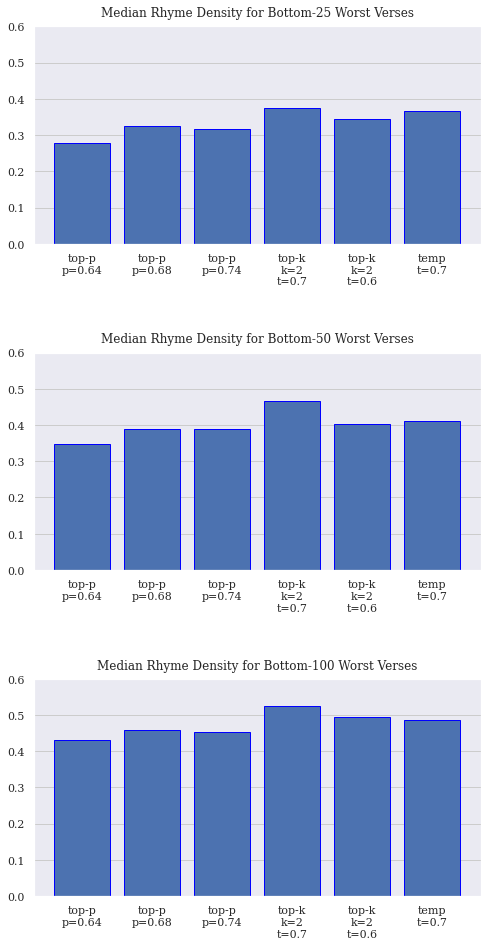
\includegraphics[scale=0.64,keepaspectratio=true]{figures/bot_verse_rd_median.png}
    \caption{Median Rhyme Density for Bottom-25, Bottom-50 and Bottom-100 Worst Verses}
    \label{fig:bot_rd_median}
\end{figure*}